\subsection{Visual Quality Calculation} \label{sec:BlurBlockSec}

Visual quality calculation is used to measure the distortion of the source image.  
Many web videos are of low quality for a variety of reasons.  
They are typically highly compressed for web-sharing, causing blurring and blocking artifacts.  
Image distortion is measured as a combination of blurriness extend and blockiness extent.

\subsubsection{Blurriness}

Our implementation of the Blurriness algorithm was based on a paper by Tong \cite{Tong}.  
The blurriness algorithm is based on the edge type and sharpness analysis using Harr wavelet transform.  
Generally edges are classified into three types; Dirac Structure, Step-Structure, and Roof-Structure.  
In the paper by Tong \cite{Tong}, Step-Structure is further classified into Astep-Structure and Gstep-Structure.   
The algorithm measures the extent of blurriness as a ratio.  The ratio is the number of likely blurred 
Gstep-Structure and Roof-Structure edges to the total number of Gstep-Structure and Roof-Structure edges.  
The classification of edges is obtained from a set of rules applied to the edge maps.  
The steps to acquire the edge maps are shown below.  
The blurriness extent is demonstrated in Figure (\ref{fig:cityOriginal}) and Figure (\ref{fig:cityBlurry}).

\vspace{5 mm}

\noindent\textbf{Step 1}: Perform Harr wavelet transform to the original image and the decomposition level is 3.  
The result is a hierarchical pyramid-like structure shown in Figure (\ref{fig:PyraStruc}).

\vspace{5 mm}

\noindent\textbf{Step 2}: Construct the edge map in each scale (i=1,2,3).
\begin{equation}
Emap_{i}(k,l)=\sqrt{LH_{i}^{2}+HL_{i}^{2}+HH_{i}^{2}}  
\end{equation}

\vspace{5 mm}

\noindent\textbf{Step 3}: Partition the edge map and find the local maxima in each window.  
The window size in the highest scale is 2 x 2, the next coarser scale is 4 x 4, and the coarsest one is 8 x 8.  
The result will be the final edge map.

\vspace{5 mm}

\begin{figure}[H] 
  \centering
  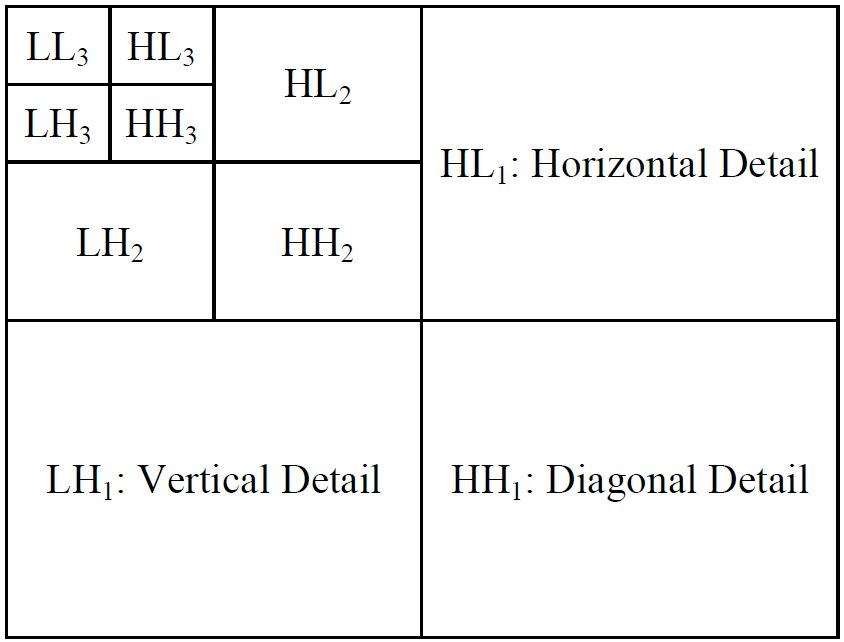
\includegraphics[scale=0.3]{pyramidStructure.jpg}  
  \caption{Pyramid of images with related sub-bands. \cite{Tong}} \label{fig:PyraStruc}
\end{figure}

\begin{figure} [H]
	\centering
	\subfigure[Blurriness = 0.2058]{
		\centering
		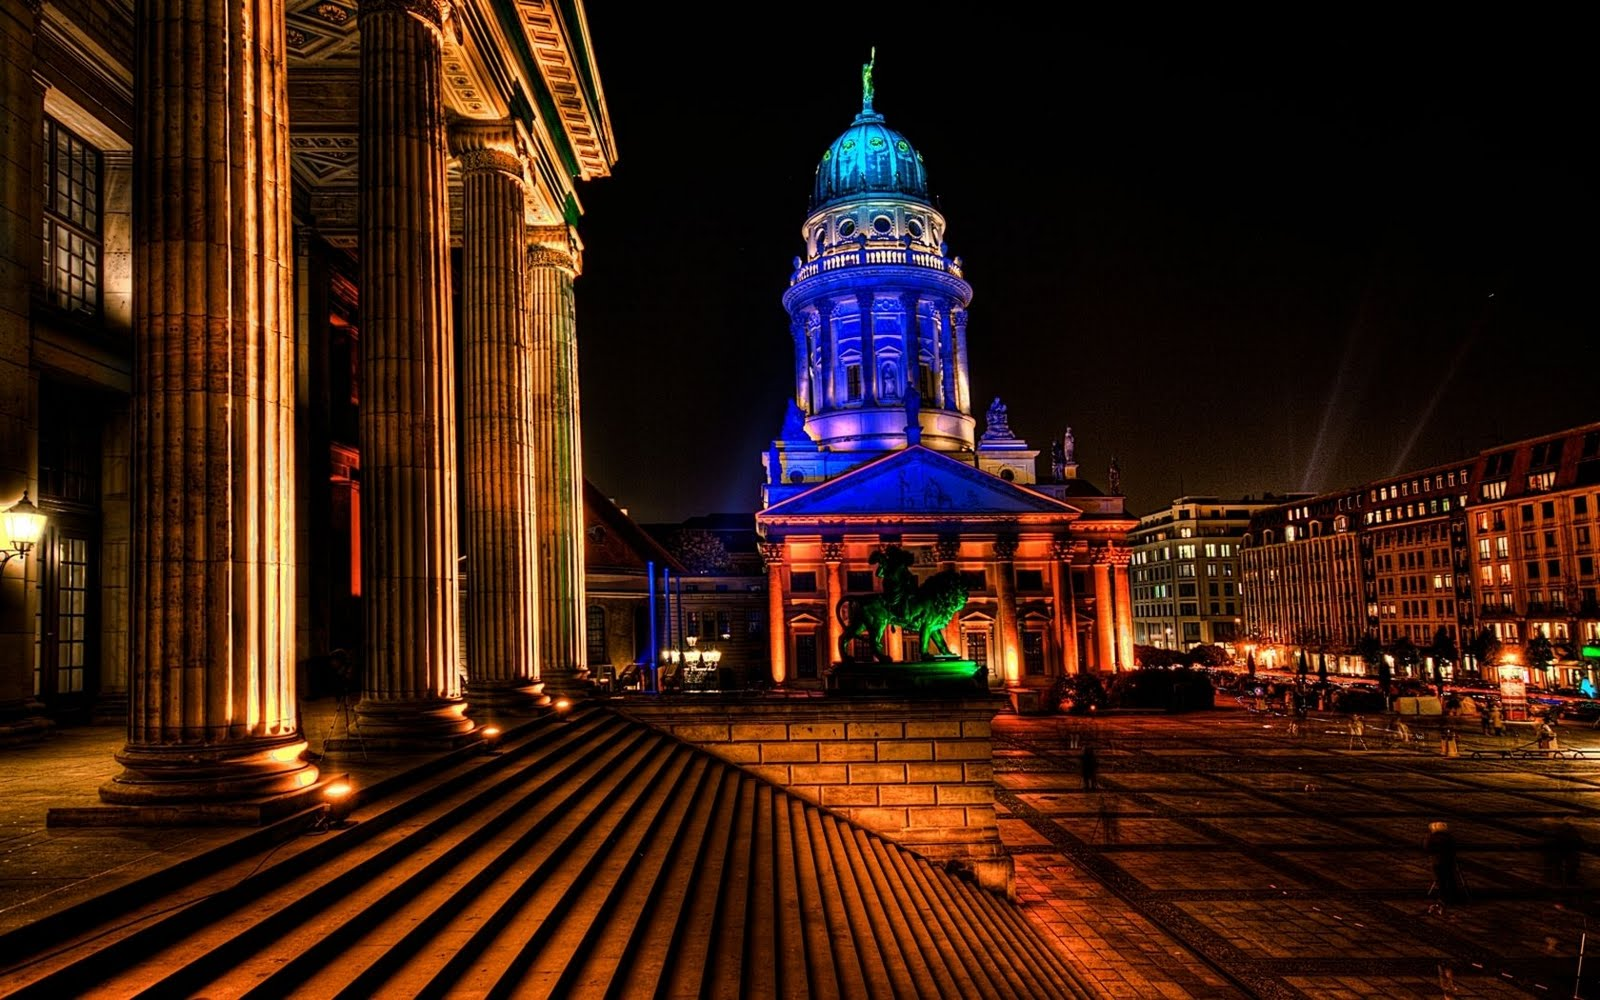
\includegraphics[width=35mm,height=35mm]{cityOriginal.jpg}  
		\label{fig:cityOriginal}	
	}
	\subfigure[Blurriness = 0.7557]{
		\centering
		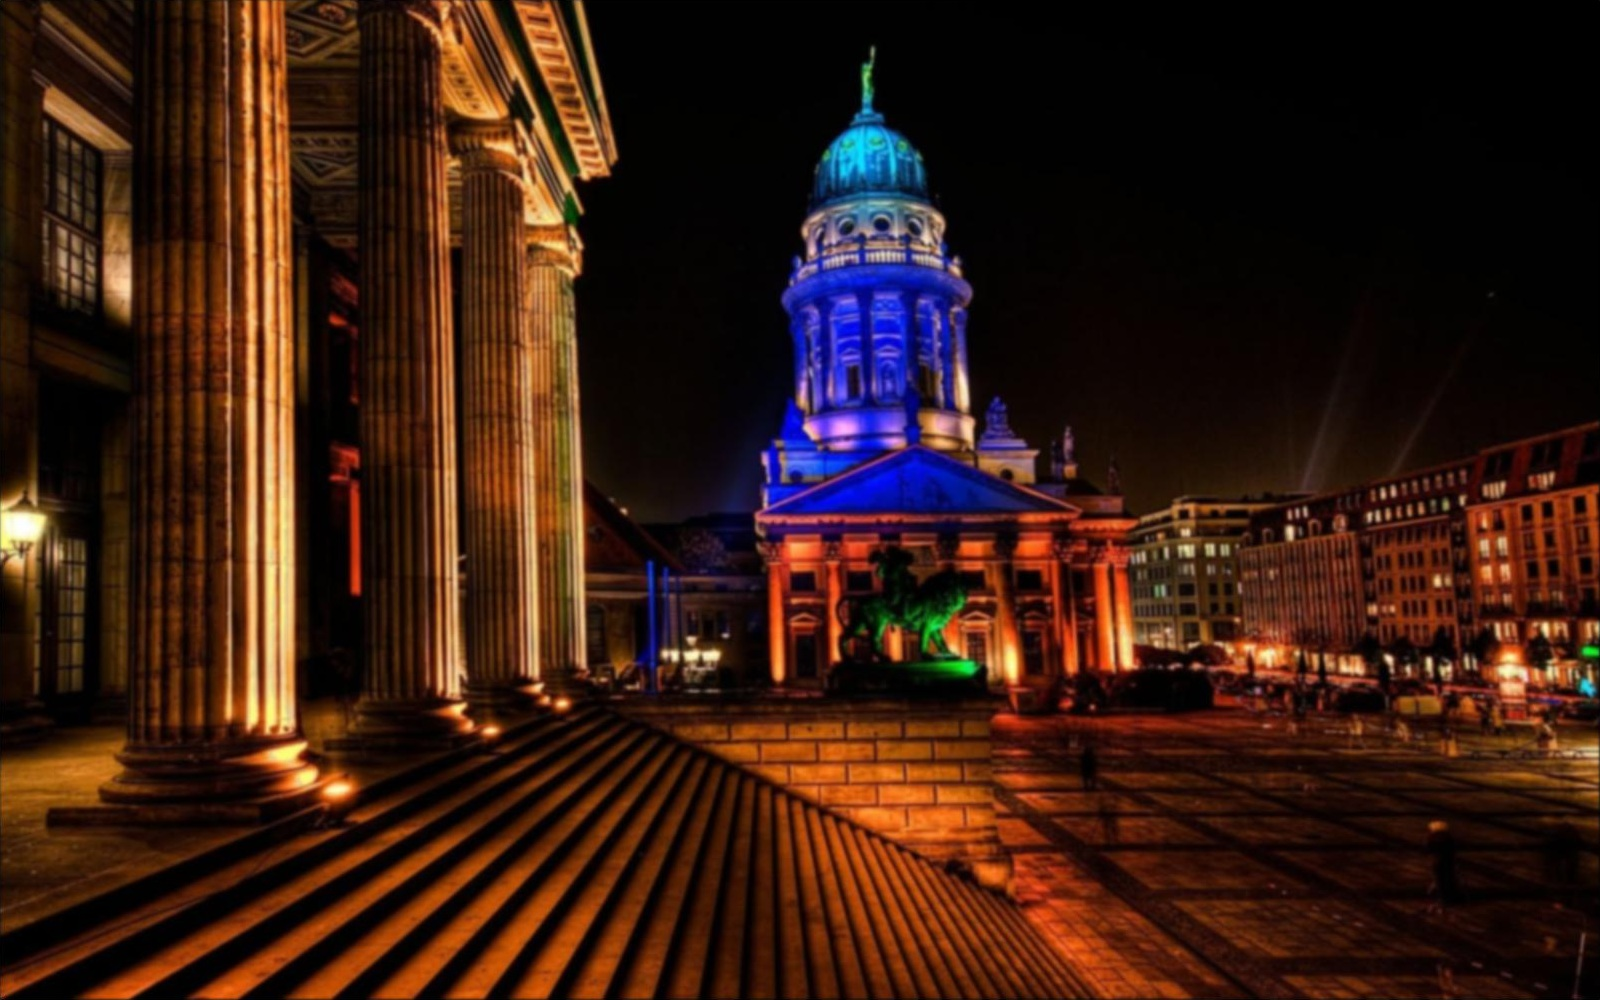
\includegraphics[width=35mm,height=35mm]{cityBlurry.jpg}  
		\label{fig:cityBlurry}
	}	
	\subfigure[Blockiness = 0.0231]{
		\centering
		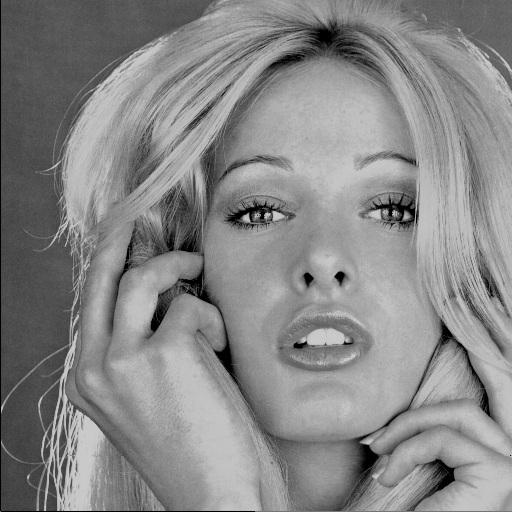
\includegraphics[width=35mm,height=35mm]{tiffanyOriginal.jpg}  
		\label{fig:tiffanyOriginal}	
	}
	\subfigure[Blockiness = 0.6744]{
		\centering
		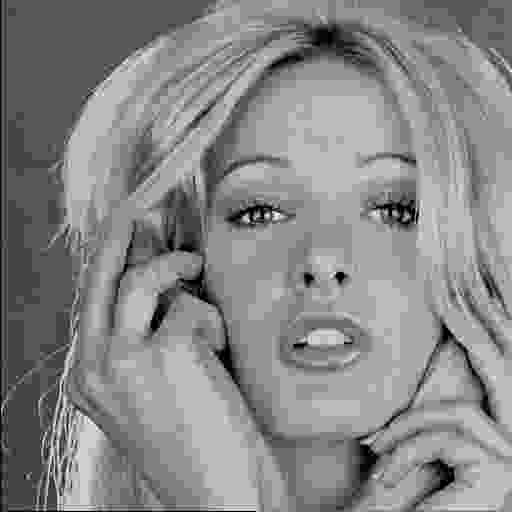
\includegraphics[width=35mm,height=35mm]{tiffanyBlocky.jpg}  
		\label{fig:tiffanyBlocky}
	}
	\caption{Blurriness and Blockiness Results.} \label{fig:BlurrBlockExp}	
\end{figure}

\subsubsection{Blockiness}

Our implementation of the Blockiness algorithm was based on a paper by Wang \cite{Wang}.  
The blockiness algorithm is designed as a No-Reference quality measurement algorithm for JPEG compressed images.  
Blockiness is estimated as the average difference across block boundaries.  
$B_{h}$ is the horizontal blockiness and $B_{v}$ is the vertical blockiness.

\begin{equation}
B_{h}=\frac{1}{M([N/8]-1)} \sum_{i=1}^{M} \sum_{j=1}^{[N/8]-1} |d_{h}(i,8j)|
\end{equation}

\begin{equation}
d_{h}(m,n)=x(m,n+1)-x(m,n)
\end{equation}

\begin{equation}
B_{v}=\frac{1}{N([M/8]-1)} \sum_{i=1}^{[M/8]-1} \sum_{j=1}^{N} |d_{v}(8i,j)|
\end{equation}

\begin{equation}
d_{v}(m,n)=x(m+1,n)-x(m,n)
\end{equation}

\noindent The final blockiness model is given in the equation below.  We used a value of 0.01 for $\beta$ and 1.0 for $\gamma$.
We also took into account the activity of the image signal as discussed in the paper \cite{Wang}.
The blockiness extent is demonstrated in Figure (\ref{fig:tiffanyOriginal}) and Figure (\ref{fig:tiffanyBlocky}).

\begin{equation}
S=\beta \left(\frac{B_{h}+B{v}}{2}\right)^\gamma
\end{equation}
















